\documentclass[11pt]{article}

\usepackage[vmargin=25mm, hmargin=20mm]{geometry}
\usepackage{parskip}
\usepackage{amsmath}
\usepackage{graphicx}
\usepackage{subcaption}

\graphicspath{ {../figures/} }

\begin{document}
\title{Machine Learning Assignment Report}
\date{\today}
\author{Ben Ellis}
\maketitle

\section*{Introduction}
% What I did
% Implemented some neural network layers using the pytorch tensors
% Implemented fully connected, CNN and MaxPool Layers
% Trained classification tasks on the iris and kmnist datasets
For this assignment I implemented the fully-connected, two-dimensional convolutional, and max pooling
neural network layers, and trained networks using these layers on two different datasets, the iris and KMNIST datasets.
I used pytorch tensors and their autograd functionality as the basis for this. 

\section*{Implementation}

\subsection*{Fully-Connected Layers, Optimisation and Initialisation}

% How I did it
% Implemented fully connected layer straightforwardly as matrix multiplication directly
% followed by a nonlinearity.
Implementing the fully connected layer can be done fairly straightforwardly as it is matrix multiplication followed by a
nonlinearity. More specifically, given input data $X$ with the shape $N \times f_{\text{in}}$ where $N$ is the size of a batch 
and $f_{\text{in}}$ is the number of features of the data coming in to the layer, the output of the layer will be 
\[
    \text{out} = g(XW)
\]
where $g$ is a function such as ReLU, sigmoid or the identity. 

% Used kaiming weight initialisation. Describe the formula here.
The weights $W$ had shape 
$f_{\text{in}} \times f_{\text{out}}$ and were initialised using Kaiming initialisation. In this form of 
initialisation, the weight tensors have values sampled from a normal distribution $\mathcal{N}(0, \sigma^2)$ where 
\[
    \sigma = \frac{\text{gain}}{\sqrt{\text{fan\_in}}}
\]
where gain is a constant determined by the particular non-linearity being used, and $\text{fan\_in}$ is the maximum
number of inputs to the layer.

For optimisation I implemented RMSProp. This divides the learning rate by a vector moving average of the gradient 
magnitudes as shown below.
\begin{align*}
    \mathbf{w}_{t} = \mathbf{w}_{t - 1} - \frac{\eta}{\sqrt{\mathbf{g}_t}} \left.\frac{\partial L}{\partial \mathbf{w}}\right|_{
        \mathbf{w} = \mathbf{w}_{t - 1}} \\
        \mathbf{g}_t = \alpha \mathbf{g}_{t - 1} + (1 - \alpha) \left.\frac{\partial L}{\partial \mathbf{w}}\right|_{\mathbf{w} = 
        \mathbf{w}_{t - 1}}
\end{align*}
where division is elementwise. There is a moving average for each weight at each layer of the same dimensions as that
weight. This means that in practice there are many moving averages. 

I tested all of the above components by using PyTorch as a reference implementation.

\subsection*{2D Convolution and Max Pooling}
% Implemented 2D convolution layer.
I also implemented 2D convolution and max pooling layers. The first of these passes a series of image patches across
each image in a batch. These can then learn to detect edges or certain colours for example. Max pooling layers take the 
maximum value in each patch. 
% Naive implementation (straight for loops in python)

The na\"ive way of implementing operations on patches like this is iterate over the rows and columns calculating either
a sum and product or a maximum. However, this is quite slow. Instead, convolutions can be implemented as matrix 
multiplication by transforming these patches into the columns of a matrix. I initially performed this naively by 
iterating over the image, but I found this too slow and so I vectorised this operation to speed it up. A comparison
of the convolution speed with this na\"ive implementation is shown in Figure \ref{tab:speed}. This shows that while the 
convolution is significantly faster than the original implementation, it is still quite a bit slower than Pytorch's 
implementation. 

\begin{table}
    \centering
\begin{tabular}{c|c|c}
    \hline 
    Na\"ive Implementation (s/it) & Faster Implementation (s/it) & Pytorch Implementation (s/it)\\
    \hline 
    0.084 & 0.015 & 0.0033 \\
    \hline

\end{tabular}
\caption{The speed of the different convolution methods in seconds per iteration on a $64 \times 16 \times 28 \times 28$
tensor. 100 repeats were timed and averaged for these results.}
\label{tab:speed}
\end{table}



\section*{Results}

In this section I present the results of training two different networks on two datasets.

\subsection*{Iris Dataset}

% IRIS dataset
% Description of data. Task is to classify iris species based on sepal length, petal length etc.
The first dataset considered is the Iris dataset. The task here is to identify different species of iris flowers 
based on their petal and sepal length and width. I trained a multi-layer perceptron with 2 layers, each with 32 nodes
to perform this task. The first layer used a ReLU nonlinearity and the second used the identity. I used the 
cross-entropy loss function. This works by first taking a softmax over the neural network outputs (to ensure that they
sum to one), and then summing $-\log p_{o, c}$ over the relevant data, where $p_{o, c}$ is the probability (according
to the neural net) that the observation $o$ is the \emph{correct} class $c$. The loss value consistently decreased 
over training as shown in Figure \ref{fig:iris}. I was also able to attain 93\% accuracy on this data, although this varies
slightly between runs.
% Architecture (2 32 wide fully-connected layers)
% Results -- 90+% accuracy. Show plot of training loss decreasing with epochs.
% Breakdown of accuracy per class. Almost all perfect.

\begin{figure}
    \centering
    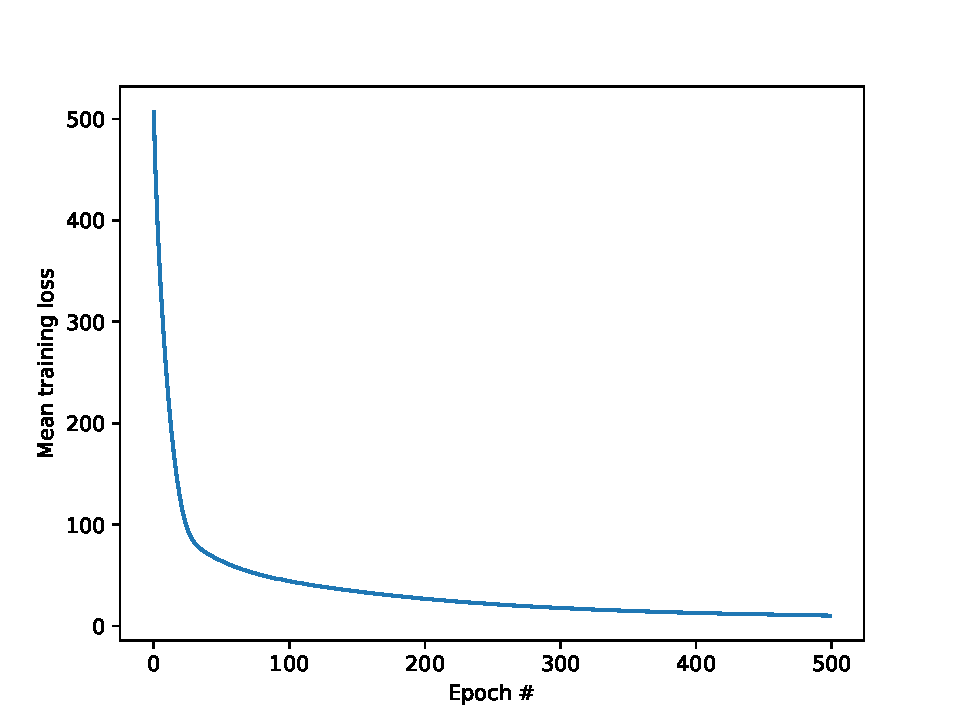
\includegraphics[width=0.5\textwidth]{Dataset.IRIS_training_loss}
    \caption{Mean loss per epoch for the IRIS dataset}
    \label{fig:iris}
\end{figure}

\subsection*{KMNIST Dataset}
% KMNIST
I also ran experiments on the KMNIST dataset. This is a dataset, designed as an alternative to MNIST, that requires
classification of japanese hiragana characters. Some examples are shown in Figure \ref{fig:kmnist}.

\begin{figure}
    \centering
    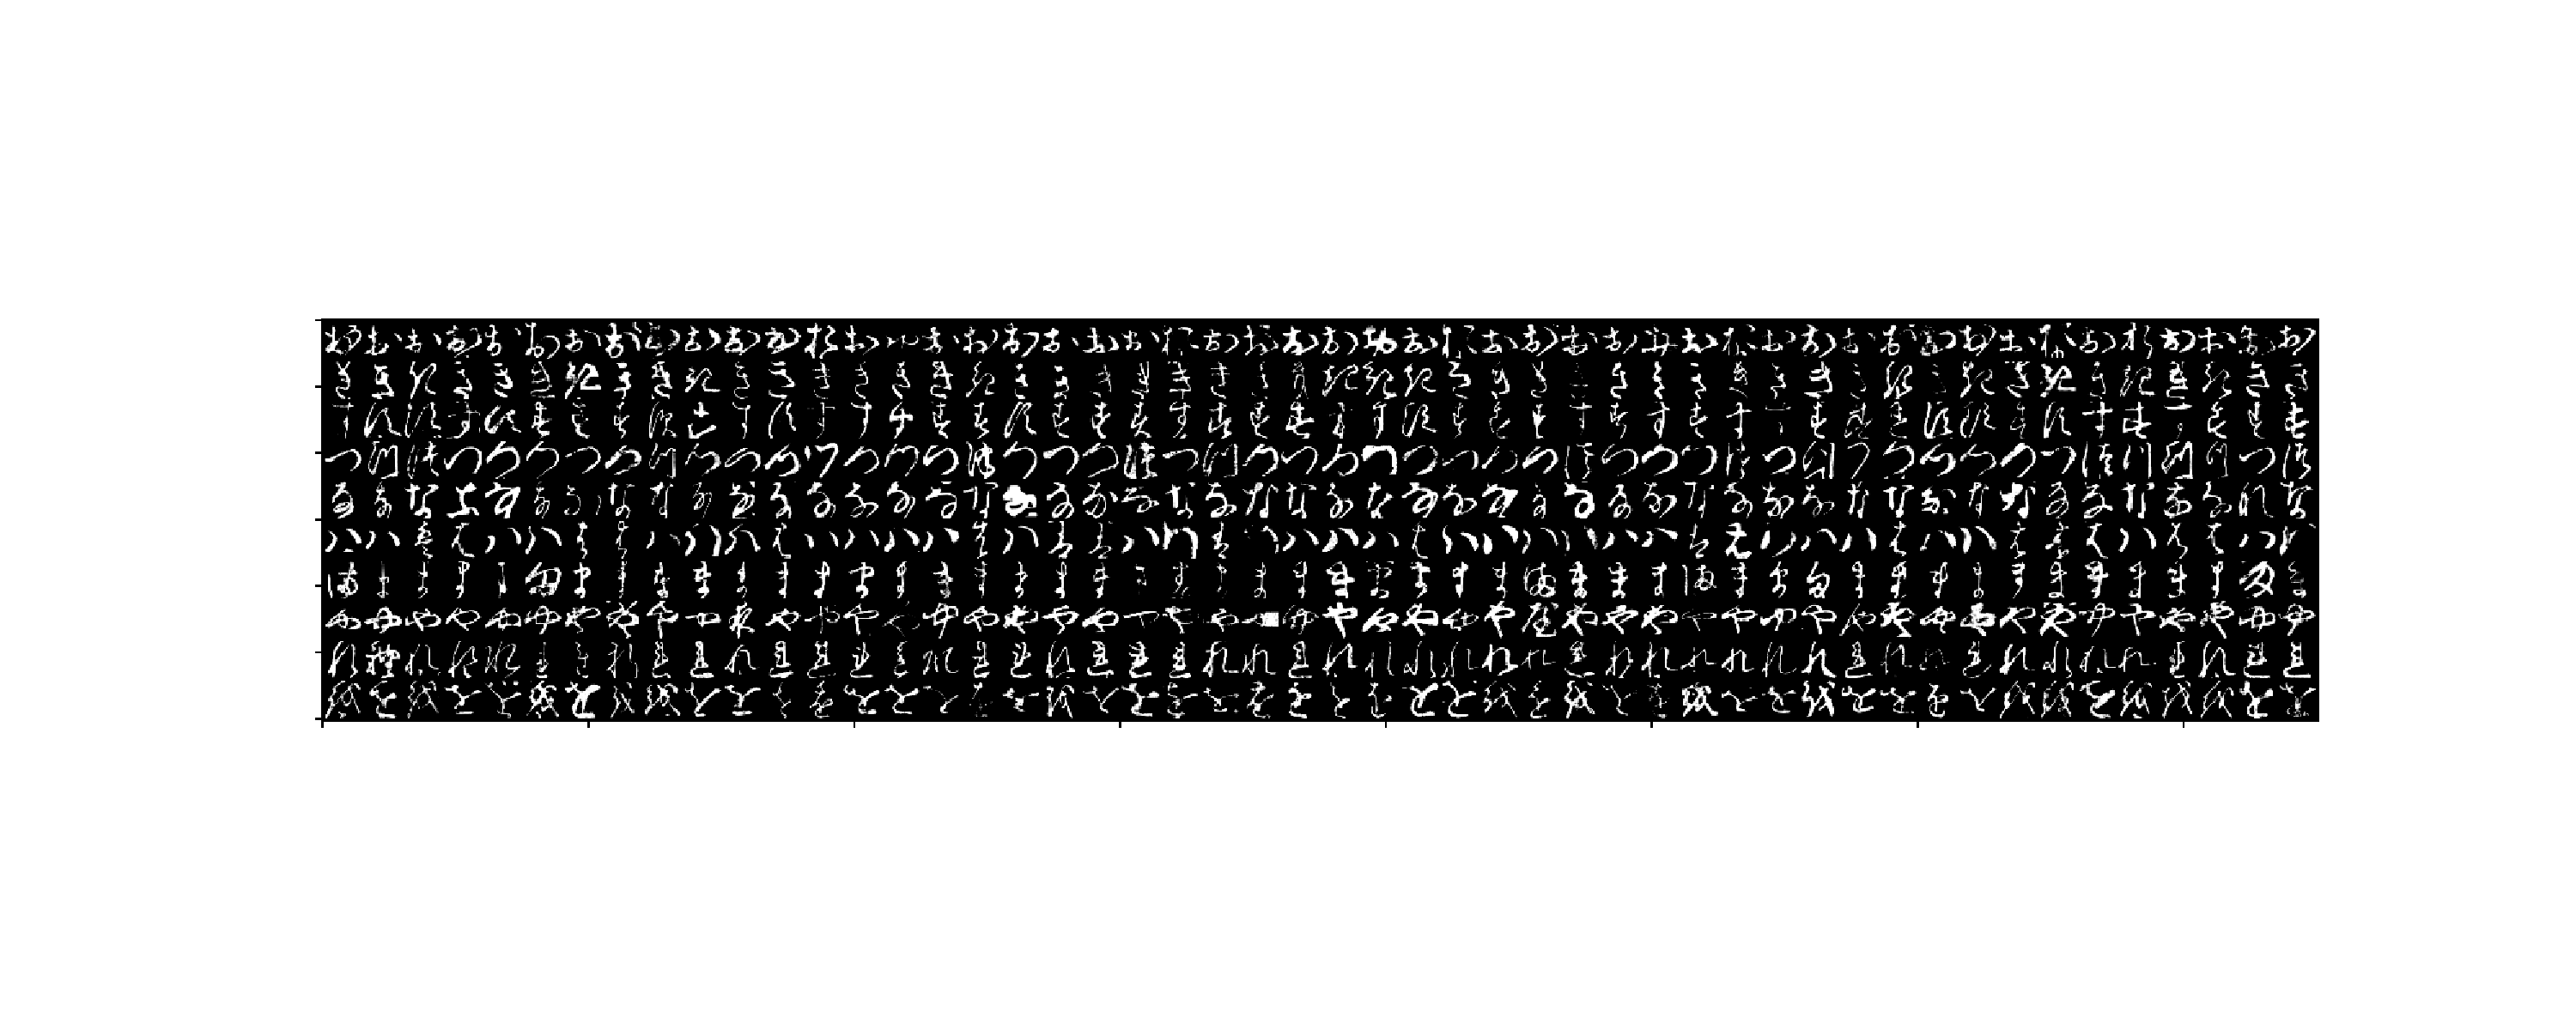
\includegraphics[width=\linewidth]{image_grid}
    \caption{Hiragana characters from the KMNIST dataset.}
    \label{fig:kmnist}
\end{figure}

I used a CNN with several layers. The first two were convolutional layers with 8 output channels and $3\times 3$ kernels.
 There was then a maxpool layer with a kernel size of 2 and a stride of 2, followed by two convolutional layers with 16 
output channels and $3 \times 3$ kernels. This was followed by a fully connected layer with 256 nodes. This was able
to attain 87.2\% accuracy on the test set. A plot of the training loss over time is shown in Figure \ref{fig:kmnist_results}, along with
 a breakdown of the accuracy per class. You can see that the classifier was particularly poor at identifying ya. This
 character looks superficially similar to some of the others such as re and some ki.

 \begin{figure}
     \begin{subfigure}{0.49\textwidth}
         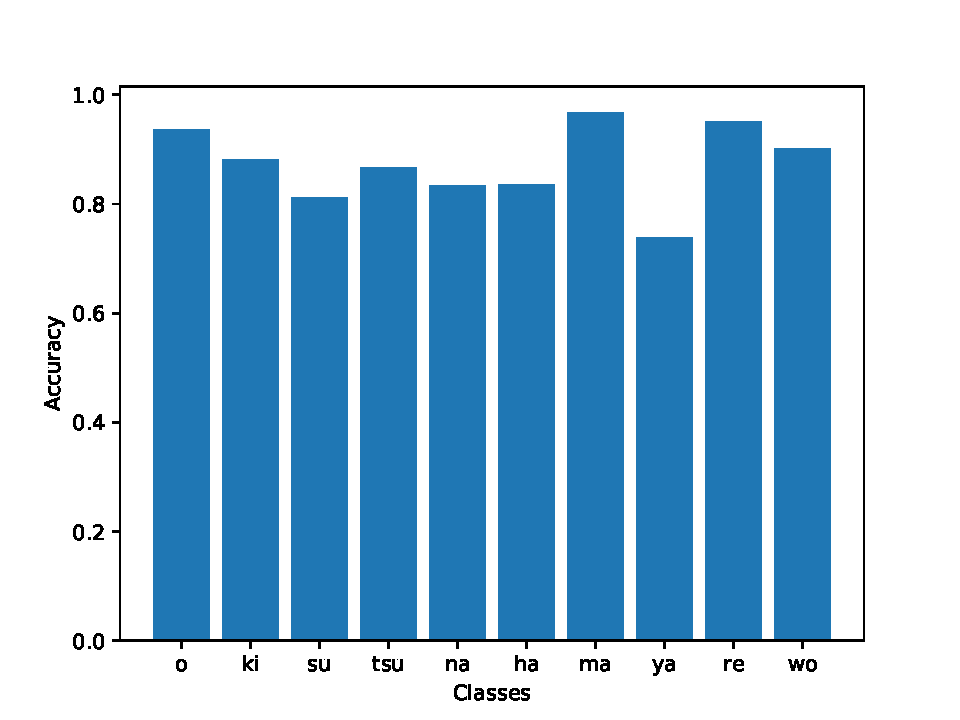
\includegraphics[width=\linewidth]{Dataset.KMNIST_classification_accuracy}
        \caption{Classification accuracy per class on the KMNIST dataset}
     \end{subfigure}
     \begin{subfigure}{0.49\textwidth}
         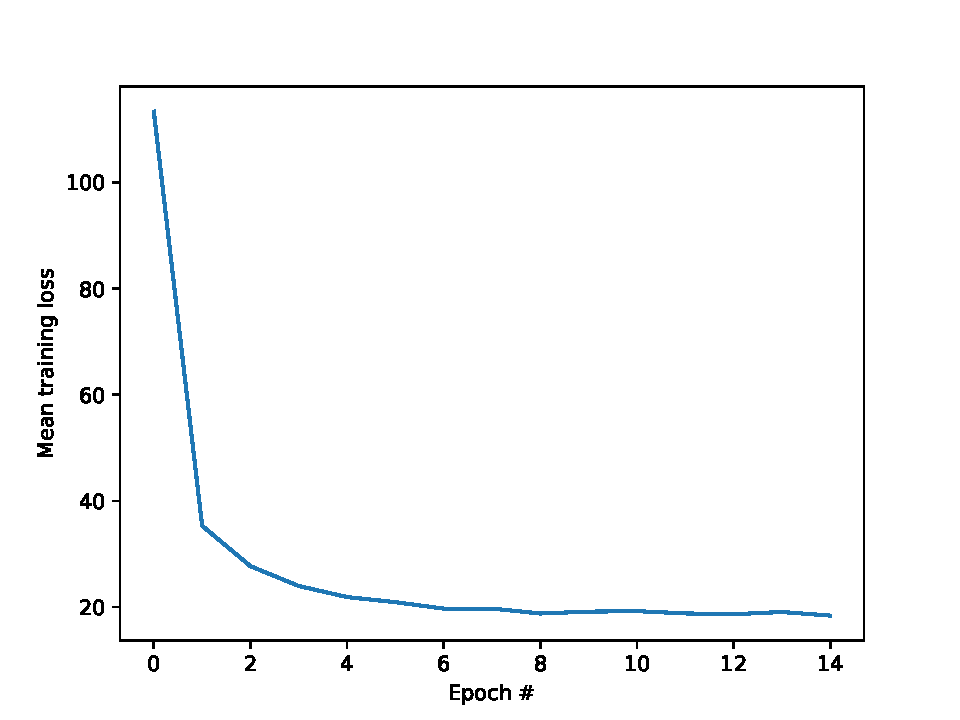
\includegraphics[width=\linewidth]{Dataset.KMNIST_training_loss}
         \caption{Mean loss per epoch for the KMNIST dataset}
     \end{subfigure}
    \caption{Results of training on the KMNIST dataset}
    \label{fig:kmnist_results}
\end{figure}
\end{document}
